% Báo cáo tiến độ 18/10/2026 — 5 trang theo yêu cầu (sửa từ bản 15/10, bản đó giữ nguyên ở bao_cao_2026-10-15).
% Cấu trúc assertion–evidence (Garner & Alley 2013): tiêu đề mỗi trang là một câu kết luận, thân trang là bằng chứng.
% Ảnh camera: episode 19 (T2, seed 1001320) của outputs/prelim/2026-10-13_slow, frame 60 (người đang chỉ tay); góc side
% dùng chung cho bộ đo và policy (thay camera high, quyết định 15/10).
% Số liệu: kiem_chung_bo_du_doan.md và outputs/dp_prediction/2026-10-18/device_stability.md (bộ đo, sim, 241 cử chỉ),
% AM của A và D (= D_f1) ghép cặp từ outputs/prelim/2026-10-13_slow/eval (scripts/fdel_report.py).
% Báo cáo tiến độ 18/10/2026 — build: latexmk (XeLaTeX, xem latexmkrc)
\documentclass[aspectratio=169,11pt]{beamer}

\usepackage{fontspec}
\setsansfont{Lato}
\newfontfamily\sym{DejaVu Sans}
\usepackage{booktabs}
\usepackage{array}
\usepackage{tikz}
\usetikzlibrary{arrows.meta,calc,positioning}
\usepackage{pgfplots}
\usepackage{graphicx}
\pgfplotsset{compat=1.18}

% ---------- màu ----------
\definecolor{ink}{HTML}{1F2328}
\definecolor{mute}{HTML}{8A9099}
\definecolor{line}{HTML}{D5DAE1}
\definecolor{accent}{HTML}{2F6FB3}
\definecolor{hot}{HTML}{E07B24}
\definecolor{ok}{HTML}{2E9E5B}

% ---------- giao diện tối giản ----------
\setbeamertemplate{navigation symbols}{}
\setbeamercolor{normal text}{fg=ink,bg=white}
\setbeamercolor{structure}{fg=accent}
\setbeamercolor{frametitle}{fg=ink}
\setbeamercolor{title}{fg=ink}
\setbeamerfont{frametitle}{size=\large,series=\bfseries}
\setbeamerfont{title}{size=\LARGE,series=\bfseries}
\setbeamertemplate{frametitle}{%
  \vspace*{0.5em}\insertframetitle\par\vspace{0.2em}%
  {\color{accent}\rule{1.2cm}{2pt}}\par}
\setbeamertemplate{footline}{%
  \hfill{\scriptsize\color{mute}\insertframenumber}\hspace*{1.2em}\vspace*{0.8em}}
\setbeamertemplate{itemize item}{\color{accent}\small$\bullet$}
\setbeamertemplate{itemize subitem}{\color{mute}\scriptsize$\bullet$}
\setlength{\parskip}{0pt}

\setbeamertemplate{title page}{%
  \vspace*{1.4cm}
  {\color{accent}\rule{1.5cm}{3pt}}\par\vspace{0.5cm}
  {\usebeamerfont{title}\usebeamercolor[fg]{title}\inserttitle\par}
  \vspace{0.35cm}
  {\large\color{mute}\insertsubtitle\par}
  \vfill
  {\insertauthor\par}\vspace{0.1cm}
  {\small\color{mute}\insertdate\par}
  \vspace*{0.9cm}}

\newcommand{\done}{{\sym\color{ok}✓}}
\newcommand{\half}{{\sym\color{hot}◐}}
\newcommand{\todo}{{\sym\color{mute}○}}
\newcommand{\gray}[1]{{\color{mute}#1}}

\title{Học chính sách hành động cộng tác\\người -- robot có nhận thức ý định}
\subtitle{Báo cáo tiến độ}
\author{Đào Duy Hưng}
\date{18/10/2026}
\newcommand{\ci}[3]{$#1$\,{\color{mute}\scriptsize[$#2$;\,$#3$]}}
\newcommand{\sig}{\textsuperscript{\color{ok}\bfseries*}}


\begin{document}

% =====================================================================
\begin{frame}[plain]
  \titlepage
\end{frame}

% =====================================================================
\begin{frame}{Hệ thống: bộ dự đoán biến cử chỉ thành ý định; chỉ robot D nhận ý định}
  \centering
  \begin{tabular}{@{}c@{\hspace{0.2cm}}c@{\hspace{0.2cm}}c@{}}
    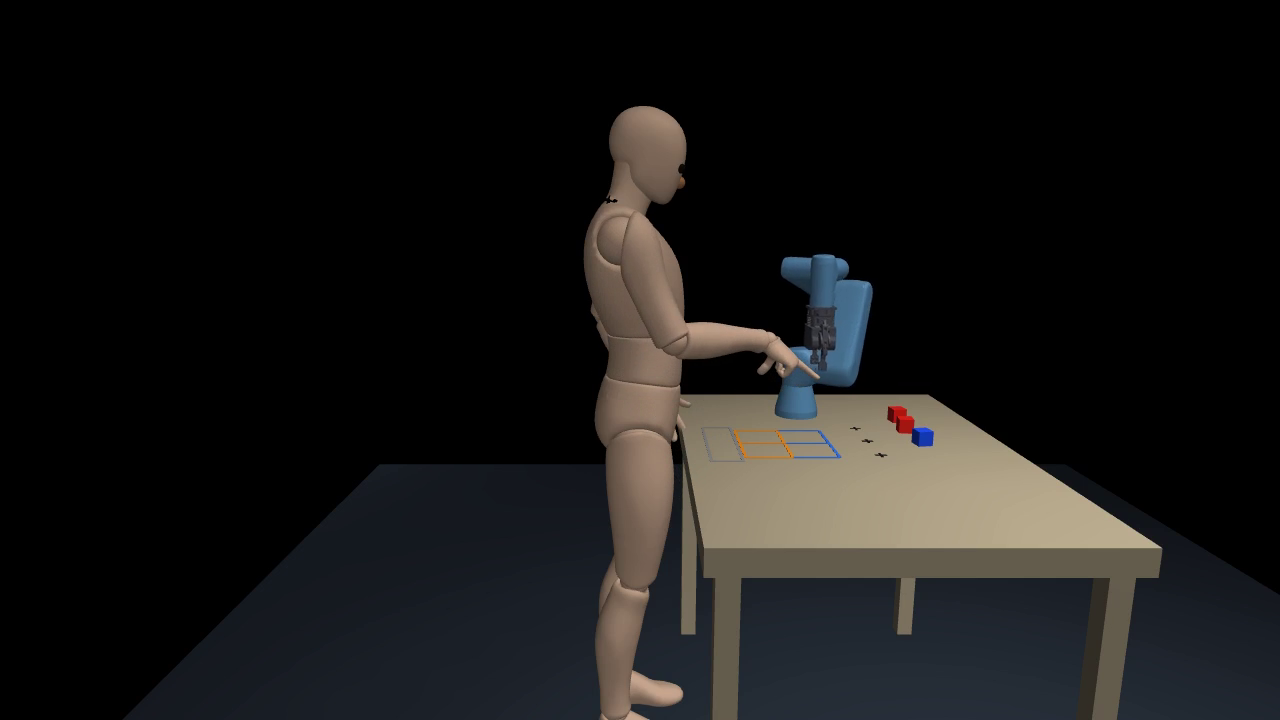
\includegraphics[height=1.55cm]{figures/cam_side.png} &
    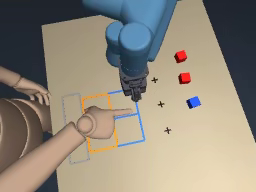
\includegraphics[height=1.55cm]{figures/cam_top.png} &
    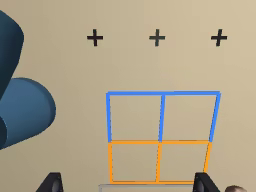
\includegraphics[height=1.55cm]{figures/cam_wrist.png} \\[-0.1em]
    \scriptsize\textbf{side}: bộ dự đoán + robot &
    \scriptsize\textbf{top}: robot &
    \scriptsize\textbf{wrist}: robot
  \end{tabular}

  \vspace{0.6em}
  \begin{tikzpicture}[
      box/.style={draw=line, rounded corners=3pt, minimum height=1.15cm, align=center, font=\small, inner sep=3pt},
      key/.style={box, draw=accent, fill=accent!8, line width=0.9pt},
      lab/.style={font=\small\bfseries, anchor=east, align=right},
      arr/.style={-{Stealth[length=5pt]}, color=mute, line width=0.8pt},
      karr/.style={-{Stealth[length=5pt]}, color=accent, line width=1.1pt}]
    % hàng 1: bộ dự đoán
    \node[lab] at (-0.25,1.45) {Bộ dự đoán};
    \node[box, minimum width=2.0cm] (in1) at (1.0,1.45) {Ảnh side\\\scriptsize 15 fps};
    \node[box, minimum width=2.8cm] (dp) at (4.0,1.45) {DeePoint\\\scriptsize cửa sổ 15 frame (1 s)\\\scriptsize cử chỉ + hướng chỉ};
    \node[box, minimum width=2.6cm] (bt) at (7.1,1.45) {Belief $b_t$\\\scriptsize FETCH-POMDP: góc\\\scriptsize giữa hướng chỉ và đích};
    \node[key, minimum width=2.4cm] (ut) at (10.1,1.45) {Ý định $u_t$\\\scriptsize xác suất từng đích\\\scriptsize + ``chờ''};
    \draw[arr] (in1) -- (dp);
    \draw[arr] (dp) -- (bt);
    \draw[arr] (bt) -- (ut);
    % hàng 2: robot
    \node[lab] at (-0.25,-0.75) {Robot};
    \node[box, minimum width=2.0cm] (in2) at (1.0,-0.75) {Ảnh 3 góc\\\scriptsize + trạng thái};
    \node[box, minimum width=2.6cm] (act) at (7.1,-0.75) {Policy ACT\\\scriptsize 40 hành động = 2 s};
    \node[box, minimum width=2.4cm] (ur) at (10.1,-0.75) {UR3e\\\scriptsize 20 Hz};
    \draw[arr] (in2) -- (act);
    \draw[arr] (act) -- (ur);
    \draw[karr] (ut.south) -- ++(0,-0.5) -| node[pos=0.27, above, font=\scriptsize, text=accent] {chỉ D} (act.north);
  \end{tikzpicture}
\end{frame}

% =====================================================================
\begin{frame}{Robot có thể bắt đầu tiến về đích khi mới thấy khoảng 30\% cử chỉ}
  \centering
  \begin{tikzpicture}[x=0.11cm, y=1cm, font=\small]
    % thanh cử chỉ 0-100%
    \fill[mute!18] (0,0) rectangle (100,0.7);
    \fill[hot!25] (0,0) rectangle (29,0.7);
    \draw[line] (0,0) rectangle (100,0.7);
    \node[font=\scriptsize, text=hot!80!black] at (14.5,0.35) {còn dao động};
    \foreach \x in {0,25,50,75,100} {
      \draw[line] (\x,0) -- (\x,-0.12);
      \node[font=\scriptsize, text=mute, below] at (\x,-0.12) {\x\%};
    }
    \node[font=\scriptsize, text=mute] at (50,-0.85) {phần cử chỉ đã thấy (100\% = tay duỗi hẳn)};
    % bắt đầu tiến
    \draw[accent, line width=1.8pt] (29,-0.15) -- (29,1.35);
    \node[font=\small, text=accent, anchor=south east, align=right] at (28.5,1.35) {\textbf{bắt đầu tiến về đích}\\\scriptsize belief $\geq 0{,}85$, ở 29\% (0,50 s)};
    % gắp
    \draw[ok, line width=1.8pt] (33,-0.15) -- (33,1.35);
    \node[font=\small, text=ok!80!black, anchor=south west, align=left] at (33.5,1.35) {\textbf{gắp}\\\scriptsize belief $\geq 0{,}9$, ở 33\% (0,60 s)};
  \end{tikzpicture}

  \vspace{1.2em}
  \small
  \begin{tabular}{@{}lcccc@{}}
    \toprule
    Ngưỡng belief & 0,7 & 0,8 & \textbf{0,85} & 0,9 \\
    \midrule
    Robot phải đổi đích sau khi vượt ngưỡng & 29\% & 15\% & \textbf{8\%} & 3\% \\
    Phần cử chỉ đã thấy (trung vị) & 19\% & 24\% & \textbf{29\%} & 33\% \\
    \bottomrule
  \end{tabular}

  \vspace{0.6em}
  \raggedright\scriptsize\gray{Ngưỡng bắt đầu tiến = mức thấp nhất mà sau khi vượt, đích dẫn đầu đổi ở dưới 10\% số cử chỉ. Sim, 241 cử chỉ bộ đo chưa thấy; một cử chỉ của người sim dài trung vị 1,75 s (đang làm chậm $\times 1{,}5$). Người thật (bộ DP) chỉ thẳng kém hơn: belief đạt 0,9 khi đã thấy khoảng 80\% cử chỉ.}
\end{frame}
% =====================================================================
\begin{frame}{Năm task, mỗi task một kiểu phối hợp; bản thử dùng T2, T3, T5}
  \centering\small
  \renewcommand{\arraystretch}{1.15}
  \begin{tabular}{@{}l>{\raggedright\arraybackslash}p{0.28\linewidth}>{\raggedright\arraybackslash}p{0.32\linewidth}>{\raggedright\arraybackslash}p{0.16\linewidth}@{}}
    \toprule
    Task & Người làm & Robot làm & Ý định đặt trên \\
    \midrule
    T1 chỉ vật & chỉ một khối, rồi chỉ chỗ đặt P1/P2 & gắp đúng khối, đặt đúng chỗ & khối; chỗ đặt \\
    \color{accent}\textbf{T2 trao vật} & chỉ một vật, rồi chìa tay ngửa ở H1/H2 & gắp vật, đưa vào lòng bàn tay, thả khi người kéo & vật; vùng tay \\
    \color{accent}\textbf{T3 cùng làm} & lấy một khối, bỏ vào cốc, ngửa tay & giữ cốc đi cặp dưới tay người, rồi đặt cốc vào tay & khối người lấy \\
    T4 an toàn & đưa tay vào vùng làm việc của robot & đứng yên khi tay trong vùng, rồi làm tiếp & không có \\
    \color{accent}\textbf{T5 đổi ý} & ra hiệu ``chờ'', rồi chọn vật kia (trên T2, T3) & dừng, đổi đích; đã cầm vật cũ thì mang trả & đích mới; ``chờ'' \\
    \bottomrule
  \end{tabular}

  \vspace{0.6em}
  \raggedright\scriptsize\gray{Ý định luôn đặt trên mục tiêu của người (ở T3 là khối, không phải cốc); khối nào đi với cốc nào robot tự học từ demo. T4 không có ý định để đoán nên dùng làm task an toàn riêng.}
\end{frame}

% =====================================================================
\begin{frame}{Robot D chốt đích sớm hơn robot A khoảng 1,2 s}
  \centering
  \begin{tikzpicture}
    \begin{axis}[ybar, bar width=34pt, width=8.2cm, height=5.6cm, ymin=-3.6, ymax=0.4,
        axis lines*=left, ymajorgrids, grid style={line},
        symbolic x coords={A,D}, xtick={A,D}, bar shift=0pt,
        xticklabels={A: demo trễ, D: demo sớm + ý định},
        ytick={-3,-2,-1,0}, yticklabels={$-3$,$-2$,$-1$,0},
        tick label style={font=\scriptsize}, label style={font=\scriptsize},
        ylabel={AM (s); âm: chốt sau khi người xong},
        nodes near coords, nodes near coords style={font=\small, color=ink, anchor=north},
        /pgf/number format/use comma, /pgf/number format/fixed, /pgf/number format/precision=2,
        enlarge x limits=0.5]
      \addplot[fill=mute!40, draw=mute] coordinates {(A,-2.95)};
      \addplot[fill=accent!60, draw=accent] coordinates {(D,-1.67)};
    \end{axis}
  \end{tikzpicture}

  \vspace{0.4em}
  \small AM = lúc người chỉ xong $-$ lúc robot chốt đúng đích. D sớm hơn A \ci{1{,}15}{0{,}90}{1{,}55} s.

\end{frame}

\end{document}
